% RaoSense — WACV 2027 main-conference working draft.
% Imaging result cells remain visibly PENDING until locked GPU runs.
\documentclass[10pt,twocolumn,letterpaper]{article}

\usepackage{../pvas_v2/wacv}
\wacvalgorithmstrack
\usepackage{times}
\usepackage{graphicx}
\usepackage{amsmath,amssymb,amsfonts,amsthm}
\usepackage{booktabs}
\usepackage{multirow}
\usepackage{algorithm}
\usepackage{algpseudocode}
\usepackage{xcolor}
\usepackage[pagebackref=true,breaklinks=true,colorlinks,bookmarks=false]{hyperref}

% \wacvfinalcopy % Keep disabled for anonymous review.
\def\wacvPaperID{****}
\ifwacvfinal\pagestyle{empty}\fi

\newcommand{\method}{RaoSense}
\newcommand{\pending}{\textcolor{red}{\textbf{PENDING}}}
\newcommand{\R}{\mathbb{R}}
\newcommand{\E}{\mathbb{E}}
\newcommand{\I}{\mathrm{I}}
\newcommand{\N}{\mathcal{N}}
\newcommand{\Cov}{\operatorname{Cov}}
\newcommand{\rank}{\operatorname{rank}}
\newcommand{\diag}{\operatorname{diag}}
\newcommand{\tr}{\operatorname{tr}}
\newcommand{\orth}{\operatorname{orth}}
\newcommand{\softmax}{\operatorname{softmax}}
\newcommand{\given}{\,\middle|\,}
\newcommand{\resultcell}{\textcolor{red}{\textbf{PEND.}}}

\newtheorem{theorem}{Theorem}
\newtheorem{proposition}{Proposition}
\newtheorem{corollary}{Corollary}

\begin{document}

\title{\method: Operator-Sufficient Diffusion Beliefs\\
for Outcome-Adaptive Imaging}
\author{Anonymous WACV submission\\Paper ID \wacvPaperID}
\maketitle

\begin{abstract}
Active imaging with diffusion priors is commonly driven by disagreement
between endpoint samples or by a single local covariance.  The former spends
many denoiser evaluations, while the latter Gaussianizes away the outcome
dependence that makes adaptive planning useful.  We introduce \method, a
compressed belief state built from a small set of measurement-guided diffusion
branches, each augmented by a low-rank local Tweedie/Jacobian factor.  Under
this finite-mixture surrogate, mutual information decomposes into an analytic
within-branch term and a bounded mode-disambiguation term.  More importantly,
all action likelihoods, information bounds, Bayesian updates, and fantasy
outcomes live in at most $\sum_k r_k+K-1$ whitened coordinates, independent of
the scalar size of an MRI line or LiDAR angular tile.  This enables
outcome-contingent horizon-two planning without additional denoiser calls and
an analytic correction that is fed back into reverse diffusion.  We also
derive a target-information extension that marginalizes low-dimensional
forward-operator nuisance instead of treating calibration as known.  Synthetic
falsification tests reduce covariance-estimation MSE by $61.6\%$, compress a
4,096-dimensional action to 11 coordinates, and recover the correct
non-myopic router.  The locked imaging study evaluates raw multicoil
fastMRI+ brain/knee data and KITTI-360 programmable LiDAR at matched
measurement and denoiser budgets.  Imaging results in this working draft are
explicitly \pending{} and will not be claimed before the preregistered
patient/drive-level gates pass.
\end{abstract}

\section{Introduction}
\label{sec:introduction}

Imaging systems rarely observe an image directly: MRI chooses k-space
trajectories, CT chooses projection angles, and programmable LiDAR chooses
angular cells.  When time, dose, or bandwidth is scarce,
the next measurement should depend on what remains uncertain for the current
subject.  Diffusion inverse solvers make this appealing
\cite{song2023pigdm,chung2023dps}: they can turn a severely
undersampled measurement into a rich conditional distribution rather than a
single reconstruction.  Yet a useful active policy must compress that
distribution, compare thousands of physically grouped actions, imagine
possible outcomes, and update the reconstruction before the next acquisition.

Diffusion acquisition methods expose a trade-off.
Particle methods use several posterior trajectories to rank measurements
\cite{nolan2025ads,elata2024adasense,morssy2024informed}.  They retain
multimodality, but endpoint disagreement is expensive and contains no
within-trajectory uncertainty.  Local Tweedie/Jacobian methods extract
posterior second moments from a denoiser
\cite{manor2024posterior,rissanen2025freehunch,schioppa2026covariance}; however,
one covariance replaces an ambiguous posterior with one Gaussian.  For a
frozen linear Gaussian belief, conditional covariance is outcome-independent,
so information planning has no advantage over open loop: the representation
removes the phenomenon adaptivity should exploit.

We ask whether a few diffusion branches and local tangent directions can
complement one another.  At an
acquisition checkpoint, branch $k$ provides a clean mean $m_k$ and a
rank-$r_k$ factor $U_k$ obtained from denoiser Jacobian-vector products.  The
resulting belief
\begin{equation}
    \widehat p(x\mid y_M)
    =\sum_{k=1}^{K} w_k\,
      \N(x;m_k,U_kU_k^\top)
    \label{eq:intro-mixture}
\end{equation}
Rao--Blackwellizes uncertainty: branch means retain global ambiguity, while
local factors integrate within-branch variation analytically.  The method
contains a particle belief when $r_k=0$ and a one-state covariance method when
$K=1$, making both failure modes explicit ablations.

Naively, a Gaussian mixture does not solve the scaling problem.  One
multicoil phase-encode line may contain tens of thousands of real scalar
measurements, and non-myopic planning appears to require repeated high
dimensional likelihoods.  Our central observation is that action $a$ depends
on the belief only through the whitened span of its pushed local factors and
branch-mean offsets.  Its dimension is at most
\begin{equation}
    d_a\leq \sum_{k=1}^K r_k + K-1,
    \label{eq:intro-rank}
\end{equation}
regardless of the number of coils, readout samples, pixels, or angular cells in the
action.  Projected fantasy observations are sufficient for component
likelihoods and exact Gaussian conditioning under the surrogate.  A
horizon-two tree therefore adds matrix and mixture operations but no denoiser
evaluation.  Figure~\ref{fig:overview} summarizes the loop.

\begin{figure*}[t]
    \centering
    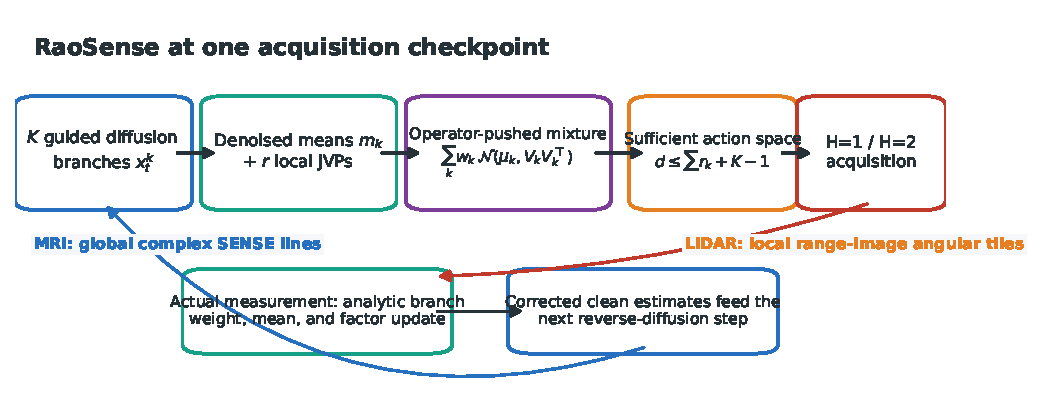
\includegraphics[width=\textwidth]{figures/method_overview.pdf}
    \caption{\textbf{\method{} loop.} A few measurement-guided reverse
    trajectories retain between-mode ambiguity; local denoiser JVPs retain
    within-mode uncertainty.  Both are pushed through the feasible operator
    bank.  Information scoring, fantasy planning, and the actual Bayesian
    update occur in a small sufficient space.  Only the real measurement is
    executed, after which corrected branch means continue through diffusion.
    The same algebra selects global complex SENSE lines and local LiDAR angular
    tiles.}
    \label{fig:overview}
\end{figure*}

The second obstacle is operator uncertainty.  Active diffusion work almost
universally assumes that the forward model is known, while blind diffusion
reconstruction estimates an operator under a fixed measurement set
\cite{chung2023blinddps,chen2025jsmoco}.  Treating uncertain coil maps, motion,
or beam geometry as known overstates how informative an action is about the
image.  We augment each local branch with a gauge-fixed nuisance factor and
derive information about the target image while marginalizing nuisance.  The
result separates measurements that resolve anatomy from measurements whose
apparent utility merely relies on perfect calibration.

The contribution is not ``Gaussian mixtures for sensing,'' ``mutual
information,'' or ``non-myopic planning'' in isolation; all are classical
\cite{braun2015infogreedy,huan2016soed,guo2026copex}.  Our claim is the
diffusion-derived \emph{operator-sufficient belief} that makes their useful
combination tractable at imaging scale.  Specifically:
\begin{itemize}
    \item We combine between-trajectory modes with within-trajectory
    Tweedie/JVP factors and preserve the mixture through acquisition and
    reconstruction updates.
    \item We derive an exact within/mode information decomposition, a lower
    and two-way upper information sandwich, safe one-step pruning, and the
    sufficient dimension bound in Eq.~\eqref{eq:intro-rank}.
    \item We implement receding-horizon outcome planning and analytic branch
    correction with no fantasy denoiser calls.  We explicitly characterize
    beam and candidate truncation as approximations, not certified pruning.
    \item We extend the objective to joint image/operator beliefs and
    preregister a two-domain evaluation on pathology-annotated raw multicoil
    MRI and programmable LiDAR, with matched NFE, prior-specific replay, and
    patient/drive-level inference.
\end{itemize}

The current synthetic results validate algebra and falsification machinery,
not imaging quality.  We retain visible placeholders rather than convert
legacy frequency-domain experiments into evidence for a different method.

\section{Related work}
\label{sec:related}

\paragraph{Adaptive sensing with generative priors.}
Informed Adaptive Sensing already uses samples from a conditional generative
model to estimate mutual information and sequentially place measurements
\cite{morssy2024informed}.  Info-Greedy sensing develops adaptive information
design for Gaussian-mixture beliefs \cite{braun2015infogreedy}.  We therefore
do not claim novelty for posterior samples, mixture beliefs, or information
greediness.  \method{} differs in how a diffusion posterior is compressed:
each partially denoised mode carries an operator-pushed local covariance, and
all downstream calculations share a provably sufficient low-dimensional
space.

ADS performs training-free active diffusion subsampling using particle
entropy during reverse diffusion \cite{nolan2025ads}.  AdaSense repeatedly
draws diffusion posterior samples and selects projected high-variance
measurements \cite{elata2024adasense}.  Iollo \etal{} formulate diffusion-guided
Bayesian experimental design for MRI and include trajectory constraints
\cite{iollo2025active}.  These establish that active diffusion imaging is
neither new nor limited to Cartesian MRI.  Our distinction is within/between
Rao--Blackwellization, analytic mixture conditioning, and compressed
outcome-contingent lookahead.  Every method is compared with measured
denoiser-call, memory, and wall-clock costs.

Zhang \etal{} optimize linear measurements through a diffusion reconstruction
loss and include a greedily ordered design \cite{zhang2025generalized}.  Their
measurements are optimized globally and fixed across test images; ours are
selected online from feasible groups using realized subject measurements.
Christoffel-DPS gives distribution-free diffusion sensor-placement theory
\cite{rowbottom2026christoffel}.  It is complementary and prevents us from
presenting local Gaussian design as universal or distribution-free.

\paragraph{Diffusion posterior moments.}
Tweedie's identity connects a denoiser Jacobian to conditional covariance
\cite{efron2011tweedie,manor2024posterior}.  Free Hunch estimates low-rank
denoiser covariance and transports it through diffusion without extra network
calls \cite{rissanen2025freehunch}; covariance-aware sampling obtains
structured posterior factors from few JVPs \cite{schioppa2026covariance}.
\method{} makes no priority claim for these identities or estimators.  Its
local factor is explicitly approximate for a learned, measurement-guided
denoiser.  The new role of the factor is as the within-mode part of an
operator-sufficient mixture used for grouped acquisition, likelihood updates,
and lookahead.

\paragraph{Sequential experimental design.}
Approximate dynamic programming, scenario trees, and online planning are
established in sequential Bayesian optimal experimental design
\cite{huan2016soed,guo2026copex}.  Our $H=2$ controller is deliberately modest:
it freezes local linearizations inside fantasies, executes only the root, and
relinearizes after the real observation.  The contribution is not planning
depth but removing image dimension and denoiser calls from every fantasy.
Immediate-information bounds safely eliminate dominated one-step leaves.
They do \emph{not} safely eliminate roots; a low-immediate action may route to
a better second measurement.  We score every root supplied to the planner and
report candidate-cap and beam truncation separately.

\paragraph{Blind and self-calibrating diffusion.}
BlindDPS runs parallel diffusion processes for an image and unknown operator
\cite{chung2023blinddps}.  JSMoCo jointly estimates MRI coil sensitivities and
motion with a self-calibrating score prior \cite{chen2025jsmoco}.  These solve
blind reconstruction for a fixed acquisition.  Conversely, active diffusion
methods generally assume a known operator.  Our target-information extension
occupies their intersection: it asks which feasible measurement is informative
about the image after marginalizing a low-dimensional operator nuisance.  We
make only a local, gauge-fixed linearization claim and include known-operator
oracle-gap and nuisance-error diagnostics.

\paragraph{MRI and LiDAR design.}
fastMRI provides raw multicoil data \cite{knoll2020fastmri}, while fastMRI+
adds non-exhaustive, single-reader pathology boxes
\cite{zhao2022fastmriplus}.  LOUPE learns static MRI sampling patterns
\cite{bahadir2020loupe}; IGS optimizes masks for medical vision tasks
\cite{razumov2023igs}.  Both are required pathology-aware static baselines.
For a genuinely different operator, R2DM supplies a public diffusion prior for
64$\times$1024 KITTI-360 range/reflectance images
\cite{nakashima2024r2dm,liao2023kitti360}.  Uncertainty-aware interactive
LiDAR sampling is already established at WACV
\cite{taguchi2023uncertainty}.  Our retrospective angular-tile study tests
whether one inference algorithm transfers from global complex Fourier lines
to local spherical coordinate groups; it is not a hardware-deployment claim.

\section{Operator-sufficient diffusion beliefs}
\label{sec:method}

\subsection{Problem and local belief}

Let $x\in\R^n$ be the target, with acquired data
$y_M=A_Mx+\epsilon_M$.  Action $a\in\mathcal A(M)$ reveals
\begin{equation}
    y_a=A_ax+\epsilon_a,\qquad
    \epsilon_a\sim\N(0,\Gamma_a).
    \label{eq:action-model}
\end{equation}
$A_a$ may be a complete complex multicoil phase-encode line in stacked real
coordinates, or selection of range/reflectance values in an angular LiDAR
tile.  $\Gamma_a$ is positive diagonal; a known whitening operator also
suffices.

At selected reverse-diffusion checkpoints, maintain $K$ trajectories
$x_t^k$ guided by $y_M$.  Their clean predictions are
$m_k=D_\theta(x_t^k,t)$.  A schedule-correct Tweedie coefficient $\kappa_t$
relates the local denoiser Jacobian to a conditional covariance surrogate.
Rather than form it in image space, we push $r_k$ candidate-space probes
through central denoiser differences.  A protected Nystr\"om factorization
produces aligned factors
\begin{equation}
 \begin{aligned}
 x\mid Z=k &\approx m_k+U_k\xi_k,\quad
 \xi_k\sim\N(0,I_{r_k}),\\[-1mm]
 \Pr(Z=k)&=w_k .
 \end{aligned}
    \label{eq:branch}
\end{equation}
The same coefficient $\xi_k$ must generate the state and every candidate
response.  This alignment, not merely matching marginal variances, is what
makes analytic conditioning possible.

For a complete candidate bank $B$, define
\begin{equation}
    \mu_k=Bm_k,\qquad V_k=BU_k.
    \label{eq:bank}
\end{equation}
Only products with $B$ and $B^\top$ are required: $B$ is full SENSE,
$(Bx)_c=\mathcal F(S_cx)$, for MRI and the identity before LiDAR tile
indexing.  Jacobian bias, finite differences, PSD projection, and imperfect
guidance make Eq.~\eqref{eq:branch} a surrogate, not an exact posterior.

\subsection{Information decomposition and bounds}

For action indices $P_a$, set
\begin{equation}
 \mu_{ka}=P_a\mu_k,\qquad
 \widetilde V_{ka}=\Gamma_a^{-1/2}P_aV_k.
\end{equation}
Under Eq.~\eqref{eq:branch},
$y_a\mid Z=k$ is Gaussian.  Information about the represented latent
$C=(Z,\xi_Z)$ decomposes as
\begin{align}
 \I(C;y_a)
 &=L_a+M_a, \label{eq:mi-decomposition}\\
 L_a
 &=\sum_k\frac{w_k}{2}
   \log\det(I+\widetilde V_{ka}^{\top}\widetilde V_{ka}),\\
 M_a&=\I(Z;y_a).
\end{align}
$L_a$ is analytic; only the categorical term is sampled from the small
predictive mixture.  Each component width comes from its local diffusion
tangent, rather than an isotropic kernel around endpoint particles.

Let $\bar\mu_a=\sum_kw_k\mu_{ka}$ and concatenate
\begin{equation}
 G_a=\left[
   \sqrt{w_k}P_aV_k,\;
   \sqrt{w_k}(\mu_{ka}-\bar\mu_a)
 \right]_{k=1}^K.
\end{equation}
The total-covariance identity gives $\Cov(P_aBx)=G_aG_a^\top$ and
\begin{equation}
 \boxed{\begin{aligned}
 L_a&\leq \I(C;y_a)\leq U_a,\\
 U_a&=\min\{U_a^{\rm G},\,L_a+H(w)\},\\
 U_a^{\rm G}&=\tfrac12\log\det
 (I+\widetilde G_a^\top\widetilde G_a).
 \end{aligned}}
 \label{eq:sandwich}
\end{equation}
where $\widetilde G_a=\Gamma_a^{-1/2}G_a$ and
$H(w)=-\sum_kw_k\log w_k$.  Thus $U_a<\max_bL_b$ safely removes $a$ for a
\emph{one-step, equal-cost} information objective.  A fixed candidate cap is
an engineering truncation and is recorded separately.

\subsection{Sufficient action coordinates}

Choose an orthonormal basis
\begin{equation}
    Q_a=\orth(\widetilde G_a),\qquad
    d_a=\rank(Q_a).
    \label{eq:q}
\end{equation}
Whiten and project an observation:
\begin{equation}
    s_a=Q_a^\top\Gamma_a^{-1/2}(y_a-\bar\mu_a).
    \label{eq:projected-observation}
\end{equation}
Coordinates orthogonal to $Q_a$ are component-independent standard Gaussian
noise and can be discarded.  In projected coordinates,
\begin{equation}
  s_a\mid k\sim\N(\delta_{ka},I+R_{ka}R_{ka}^\top),
\end{equation}
with
\begin{equation}
  \delta_{ka}=Q_a^\top\Gamma_a^{-1/2}(\mu_{ka}-\bar\mu_a),
  \quad R_{ka}=Q_a^\top\widetilde V_{ka}.
\end{equation}
Thus $d_a\leq\sum_kr_k+K-1$.  Numerical SVD truncation is approximate if it
drops a nonzero direction; we log rank and tolerance.

\subsection{Outcome update and reverse diffusion}

For either a fantasy or real $s_a$, component $k$ updates in coefficient
space:
\begin{align}
 \Lambda_{ka}&=(I+R_{ka}^\top R_{ka})^{-1},\\
 \widehat\xi_{ka}
 &=\Lambda_{ka}R_{ka}^\top(s_a-\delta_{ka}),\\
 m_k^+&=m_k+U_k\widehat\xi_{ka},\qquad
 U_k^+=U_k\operatorname{chol}(\Lambda_{ka}), \label{eq:update}\\
 w_k^+&\propto w_k\,
 \N(s_a;\delta_{ka},I+R_{ka}R_{ka}^\top).
\end{align}
The same update changes every unobserved candidate mean through
$V_k\widehat\xi_{ka}$.  After a real observation, $m_k^+$ enters the next
deterministic reverse step.  For VP/DDIM~\cite{song2021ddim},
\begin{equation}
 x_{t'}^k=\alpha_{t'}m_k^+
 +\sigma_{t'}\frac{x_t^k-\alpha_tm_k}{\sigma_t}.
 \label{eq:ddim-update}
\end{equation}
The implementation then re-evaluates the denoiser at the next ordinary step.

\subsection{Receding-horizon planning}

The $H=2$ value of root $a$ is
\begin{equation}
 Q(a)=g_b(a)+\gamma\E_{s_a}
 \left[\max\{0,\max_{a'\in\mathcal A(a)}g_{b^+(s_a)}(a')\}\right],
 \label{eq:h2}
\end{equation}
where $g_b(a)=\I_b(C;y_a)-c_a$.  Projected fantasies use
Eqs.~\eqref{eq:projected-observation}--\eqref{eq:update}, so the tree calls no
denoiser.  The confirmatory configuration supplies and scores every feasible
root, then expands an immediate-utility beam, executes one root, and replans
after its outcome.  The expansion beam is heuristic; any root cap is a
separately labeled engineering ablation.  Immediate bounds safely prune
equal-cost future leaves, never roots, and all-expansion small-scale runs
measure beam sensitivity.

\begin{algorithm}[t]
\caption{\method{} at one acquisition checkpoint}
\label{alg:raosense}
\begin{algorithmic}[1]\footnotesize
\Require states $\{x_t^k,w_k\}$, acquired data $y_M$, feasible groups
\For{$k=1,\ldots,K$}
  \State $m_k\gets D_\theta(x_t^k,t)$; obtain aligned $(U_k,V_k)$
\EndFor
\State build mixture bounds and projected action models
\State score every feasible root; expand $H=2$ beam with projected fantasies
\State acquire only $a^\star$ and observe real $y_{a^\star}$
\State update $\{w_k,m_k,U_k\}$ analytically by Eq.~\eqref{eq:update}
\State continue each branch by Eq.~\eqref{eq:ddim-update}
\end{algorithmic}
\end{algorithm}

\subsection{Target information under operator nuisance}
\label{sec:target-information}

Let $\phi$ be a low-dimensional nuisance in
$y_a=A_a(\phi)x+\epsilon$.  Linearizing around $(m_k,\bar\phi_k)$ gives
\begin{equation}
  y_a\approx A_a(\bar\phi_k)x+
  \left[\partial_\phi A_a(\bar\phi_k)m_k\right](\phi-\bar\phi_k)+\epsilon.
  \label{eq:nuisance-linearization}
\end{equation}
Append a gauge-fixed nuisance factor to each branch.  For one branch, write
the whitened response as
$R_x\xi_x+R_\phi\xi_\phi+e$, initially with independent image and nuisance
coefficients.  Information about the image while marginalizing nuisance is
\begin{equation}
 \I(\xi_x;y_a\mid k)
 =\tfrac12\log\frac{
   \det(I+[R_x,R_\phi]^\top[R_x,R_\phi])}{
   \det(I+R_\phi^\top R_\phi)}.
 \label{eq:target-info}
\end{equation}
After conditioning rotates coefficient directions, we instead use the null
space of the target-state factor.  For a mixture, target $(Z,x)$ retains the
mode term:
\begin{equation}
 \I(Z,x;y_a)
 =\I(Z;y_a)+\sum_kw_k\I(x;y_a\mid Z=k).
 \label{eq:mixture-target}
\end{equation}
This rewards mode/anatomy resolution while treating calibration variation as
structured noise.  Because label information counts, $Z$ must be
target-relevant; nuisance-only or duplicate labels can overcount image
information.  Label-marginalized $\I(x;y_a)$ is not implemented.  This does
not prove global blind identifiability; nuisance bases remain low-dimensional
and gauge-fixed.

\section{Guarantees and approximation boundary}
\label{sec:theory}

Results below hold for the finite local mixture in Eq.~\eqref{eq:branch};
they do not certify calibration to the true diffusion posterior.

\begin{proposition}[Mixture covariance factor]
Let $\bar m=\sum_kw_km_k$.  Then
\begin{equation}
 \Cov(x)=LL^\top,\quad
 L=\left[\sqrt{w_k}U_k,\sqrt{w_k}(m_k-\bar m)\right]_{k=1}^K.
\end{equation}
Moreover, $\rank(L)\leq\sum_kr_k+K_+-1$, where $K_+$ is the number of
positive-weight branches.
\end{proposition}
\noindent
This is total covariance.  The mean offsets sum to zero, giving $K_+-1$;
pushing $L$ through an action gives $G_a$ and the same bound.

\begin{theorem}[Information sandwich]
Under independent Gaussian action noise, Eq.~\eqref{eq:mi-decomposition} is
exact for the represented latent $C$.  Its information satisfies
Eq.~\eqref{eq:sandwich}.
\end{theorem}
\noindent
The chain rule gives
$\I(Z,\xi_Z;y)=\I(Z;y)+\I(\xi_Z;y\mid Z)$.  The latter is a weighted
linear-Gaussian log determinant.  Nonnegativity and
$\I(Z;y)\leq H(Z)$ give the lower bound and entropy cap.  A Gaussian maximizes
entropy at fixed covariance, giving the moment-Gaussian upper bound.

\begin{corollary}[Safe one-step screening]
For an equal-cost one-step objective, if $U_a<\max_bL_b$, action $a$ is not
optimal under the mixture surrogate.
\end{corollary}
\noindent
This does not apply to an $H=2$ root: future value may reverse the immediate
ordering.  Confirmatory paired $H=1/H=2$ runs score all roots through the same
estimator; screening remains an optional $H=1$ primitive.

\begin{theorem}[Operator sufficiency]
Let $Q_a$ span $\widetilde G_a$ exactly.  The projected observation $s_a$ in
Eq.~\eqref{eq:projected-observation} is sufficient for the component label and
local coefficient.  Hence it preserves mixture likelihood ratios, mutual
information, and the posterior update, with
\begin{equation}
 \dim(s_a)\leq\sum_kr_k+K_+-1.
\end{equation}
\end{theorem}
\noindent
After whitening, a vector orthogonal to $Q_a$ removes all factors and mean
offsets, leaving standard Gaussian noise independent of $(Z,\xi_Z)$.
Factorization gives sufficiency.  The numerical SVD implementation is
approximate if it drops a nonzero singular value.

\begin{proposition}[No outcome adaptivity for one Gaussian]
For one frozen linear-Gaussian component, independent Gaussian measurements,
and outcome-independent feasibility/costs, an optimal finite-horizon
expected-information policy can be chosen open loop.
\end{proposition}
\noindent
Posterior covariance depends on selected actions, not their values, so
backward induction yields an action-history-only continuation.  In \method{},
adaptive value can arise from updated mode weights/means, relinearization,
operator uncertainty, or outcome-dependent constraints.

\paragraph{Conditional $H=2$ error statement.}
Let $\mathcal B$ be the retained root beam, let
$\Delta_{\mathcal B}=\max_aQ(a)-\max_{a\in\mathcal B}Q(a)$, and suppose every
estimated root, future action, and fantasy expectation is uniformly accurate
within $\varepsilon_0,\varepsilon_1,\varepsilon_F$, respectively.  Then the
selected root $\widehat a$ obeys
\begin{equation}
 \max_aQ(a)-Q(\widehat a)
 \leq\Delta_{\mathcal B}
 +2[\varepsilon_0+\gamma(\varepsilon_1+\varepsilon_F)].
 \label{eq:regret}
\end{equation}
This follows from the 1-Lipschitz maximum and empirical-argmax inequalities.
It is conditional, not a finite-sample certificate: mixture information
density has an unbounded negative tail, nested maxima are biased, and
$\Delta_{\mathcal B}$ is unbounded here.  Monte Carlo errors are descriptive;
cap/beam sensitivity is tested empirically.

\paragraph{Complexity.}
With $T$ reverse steps, $K$ branches, $J$ acquisition rounds, and rank $r$,
central differences use
\begin{equation}
    KT+2KrJ
    \label{eq:nfe}
\end{equation}
image-equivalent denoiser evaluations.  Planning adds zero NFE but nonzero
wall time.  Headline $K=8,r=2,T=32,J=4$ uses 384 NFE, matching a
$K=12,T=32$ point ensemble.  Perturbations and branches are batchable, but we
report calls, launches, memory, and latency.

\section{Locked experimental design}
\label{sec:experiments}

All real-data cells are frozen before production.  Protocols, manifests, and
the A800 notebook accompany the code.  We separate native reconstruction from
passive replay of the final mask.  Replay isolates selection only within a
fixed prior; comparing policies with different learned priors requires an
additional, independently trained replay prior.  Native quality, angular
queries/MRI lines, NFE, latency, launches, and memory are reported separately.

\subsection{Raw multicoil fastMRI+}

\paragraph{Cohorts and split.}
We join raw multicoil fastMRI brain/knee acquisitions
\cite{knoll2020fastmri} by filename to fastMRI+ lists and boxes
\cite{zhao2022fastmriplus}: 1,001 reviewed brain and 1,172 knee studies.
Single-reader, non-exhaustive labels are annotated regions, not diagnostic
ground truth.  HDF5 files are SHA256-pinned; slices stay within study, and
patient identity is used only when auditable under the data agreement.

Grouped multilabel folds assign 50\% to prior/detector/baseline training,
16.7\% to calibration, and 33.3\% to locked testing.  No slice crosses folds.
Public checkpoints are smoke-test-only without a disjoint training manifest;
the confirmatory track trains fresh anatomy-specific priors.

\paragraph{Measurement protocol.}
The primary cell starts at nominal $R=8$ with 4\% ACS and adds 16 complete
phase-encode columns.  At each of four diffusion checkpoints it selects four
columns \emph{sequentially}, conditions after every observed line, and replans:
there are 16 feedback opportunities but only four tangent refreshes.  A
$4\times4$ packet ablation selects four lines without within-packet feedback.
Each action contains every coil/readout sample in one column.  Sensitivities
and normalization use acquired ACS only; policies share mask, hidden
measurement field, estimate, and seed.  Secondary budgets are $\{8,24\}$
lines and $R=4$.

\paragraph{Clinical endpoints.}
We report volume RSS NMSE, PSNR, SSIM, HFEN, and LPIPS, plus box and
size-matched normal-patch versions.  Because annotation export vertically
flipped images, ten overlays are manually checked.  A frozen detector is
cross-fitted by patient/study from fully sampled references; mAP, common-class
sensitivity, hallucination errors, and worst deciles are reported.  Resampling
uses patient/study, never slices or boxes.

\subsection{KITTI-360 programmable LiDAR}

R2DM \cite{nakashima2024r2dm} maps KITTI-360
\cite{liao2023kitti360} to a 64$\times$1024 range/reflectance raster.  Its
public checkpoint supports reproduction; confirmation uses a fresh prior and
held-out drives.  We select 5,000 deterministic temporally thinned test frames
from drives 0 and 2, reporting drives separately.

Every method starts with a 12.5\% scout: all rows at every eighth azimuth.
A 4$\times$128 tile contains 512 angular cells, 64 already scouted, so an
action reveals 448 new range-image queries (896 scalar fields).  As in MRI,
four checkpoints each make four sequential, outcome-conditioned selections:
16 feedback opportunities end at 15,360 observed angular cells (23.44\%).
The $4\times4$ no-within-packet-feedback variant is an ablation.  These cells
are not verified physical laser firings.  The headline likelihood models only
the two continuous R2DM channels, where invalid cells carry sentinel $-1$.
The separate validity tensor is evaluation-only, never a third planner
observation.  Likelihood variance $10^{-3}$ is a numerical regularizer, not
sensor noise; noisy/no-return robustness remains pending.  This is
retrospective beam emulation, not hardware validation.

Metrics include valid-return range/reflectance MAE, distance bins,
point-cloud distance, BEV occupancy IoU, and RangeNet mIoU against aligned
held-out semantics.  Network predictions on full scans are not ground truth.
Inference uses temporal blocks and drive-stratified effects.

\begin{table*}[t]
\centering
\caption{\textbf{Confirmatory comparison set.} Canonical replay uses one
32-step solver within each fixed-prior arm; an independent replay prior is
required for cross-prior mask claims.  Exact NFE uses measured counters.}
\label{tab:baselines}
\small
\setlength{\tabcolsep}{4pt}
\resizebox{\textwidth}{!}{%
\begin{tabular}{lllll}
\toprule
Family & MRI & LiDAR & Training / privileged input & Comparison role\\
\midrule
Static & equispaced, VD random & uniform, random tiles & none & budget controls\\
Learned static & LOUPE, IGS & calibration-fixed tiles & domain/task training & strong nonadaptive\\
Learned active & uncertainty/RL MRI policy & interactive LiDAR & policy training; may use RGB & separate privileged tier\\
Diffusion active & ADS, AdaSense, Iollo BED & ported ensemble variance & same prior and actions & closest published family\\
Point belief & $K=12,16$ ensembles & $K=12,16$ R2DM ensembles & no policy training & in-family controls\\
Local Gaussian & SketchSense ($K=1$) & SketchSense ($K=1$) & no policy training & removes modes\\
\method{} & $H=1$ and $H=2$ & $H=1$ and $H=2$ & no policy training & proposed comparison\\
Diagnostic & hidden-target greedy & hidden-target greedy & target access & nondeployable ranking check\\
\bottomrule
\end{tabular}
}
\end{table*}

\subsection{Baselines, fairness, and ablations}

Table~\ref{tab:baselines} lists the minimum comparison set.  Morssy-style
empirical sample MI is included even if reimplemented, because generative
sample MI predates our work \cite{morssy2024informed}.  Static pathology-aware
MRI masks include LOUPE and IGS \cite{bahadir2020loupe,razumov2023igs}.
LiDAR includes the WACV interactive-sampling baseline
\cite{taguchi2023uncertainty}.  If a method originally chooses arbitrary
Fourier points, its legal full-line port is labeled as such.

The exact-NFE headline compares \method{} $K=8,r=2$ with the in-family
$K=12,r=0$ point ensemble at 384 NFE.  $K=16$ is a 512-NFE in-family
quality/memory reference, not a faithful ADS or AdaSense reproduction.
Calibration selects wall-clock variants within $\pm5\%$ latency on one A800;
a second GPU runs an independent anatomy/drive shard.

Load-bearing ablations are $K\in\{1,4,8,16\}$,
$r\in\{0,1,2,4\}$, $H\in\{1,2\}$, equal versus updated weights,
selection-only versus correction-only versus both, exact mixture versus
moment-Gaussian upper scoring, matched-compute extra particles, candidate cap
$C\in\{48,96,\text{all}\}$, beam width, fantasy count, and fresh versus
transported factors.  Confirmatory H1 and H2 both receive all feasible roots,
use the same seed/estimator path (H1 sets future discount to zero), and differ
only in future value.  Any root cap or finite H2 expansion beam is explicitly
heuristic; all-expansion small cases measure sensitivity.  We report changed
roots and realized retrospective two-step value.

\subsection{Operator-nuisance stress}

MRI stressors are gauge-fixed global coil gain/phase and piecewise-rigid line
motion; LiDAR stressors are elevation zero-offset and range gain/bias.
Comparisons include image-only \method{}, target-information \method{},
fixed-mask blind reconstruction, known-operator oracle, and random/equispaced
acquisition.  We report nuisance error, image/task quality, worst decile, and
the fraction of the known-operator oracle gap recovered.  The nuisance model
is fitted on calibration data only.  This study is promoted to a headline
claim only if the local linearization remainder and gauge diagnostics pass.

\paragraph{Inference.}
Primary effects pair patients/studies or temporal blocks.  We report paired
bootstrap 95\% intervals and preregistered one-sided Wilcoxon/permutation
tests with Holm correction.  Slice/frame curves are descriptive; excluded
locked cases retain fold and reason.

\section{Results and falsification gates}
\label{sec:results}

\subsection{Analytic checks completed}

Figure~\ref{fig:analytic} and Table~\ref{tab:analytic} are non-imaging checks.
For a known synthetic mixture, Rao--Blackwellization reduced covariance MSE
from 0.3746 to 0.1440 at the declared sample budget.  A 4,096-scalar action
used 11 sufficient coordinates (372.4$\times$ compression), and estimated MI
$4.1573\pm0.0039$ nats (Monte Carlo SE) lay within
$[2.8694,4.2557]$.  A six-mode case selected the correct $H=2$ binary router
instead of the myopic ternary action.  These test identities, not diffusion
calibration or real-image quality.

\begin{figure*}[t]
    \centering
    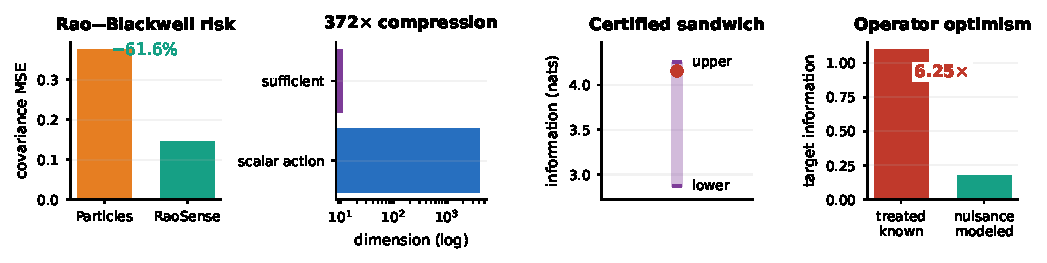
\includegraphics[width=.94\textwidth]{figures/analytic_validation.pdf}
    \caption{\textbf{Completed synthetic checks.} Left to right:
    Rao--Blackwell covariance risk; action-space compression; mutual
    information estimate and certified surrogate bounds; and the target
    information lost when operator nuisance is modeled instead of assumed
    known.  No panel is a real imaging result.}
    \label{fig:analytic}
\end{figure*}

\begin{table}[t]
\centering
\caption{Completed analytic evidence.  SE is descriptive Monte Carlo error,
not a nested-planning confidence certificate.}
\label{tab:analytic}
\small
\begin{tabular}{lc}
\toprule
Check & Observed value\\
\midrule
Particle covariance MSE & 0.3746\\
Rao--Blackwell covariance MSE & 0.1440\\
Scalar / sufficient dimension & 4096 / 11\\
MI lower / estimate / upper & 2.869 / 4.157 / 4.256\\
Myopic root / $H=2$ root & 0 / 1\\
Target MI, nuisance unknown / known & 0.176 / 1.099\\
\bottomrule
\end{tabular}
\end{table}

\subsection{Locked imaging tables}

Table~\ref{tab:primary-results} is intentionally unfilled.  Canonical replay
isolates masks within a fixed prior; a cross-prior claim requires an
independent replay prior.  Native quality is separate.  Calibration, never
test metrics, chooses the strongest active comparator.

\begin{table*}[t]
\centering
\caption{\textbf{Locked primary imaging results.} All entries remain
\resultcell{} until frozen GPU artifacts, provenance, and clustered inference
pass review.  MRI is volume-level at $R=8$ plus 16 lines; LiDAR is
drive/block-level at 15,360 angular cells.  Arrows indicate direction.}
\label{tab:primary-results}
\scriptsize
\setlength{\tabcolsep}{3.2pt}
\renewcommand{\arraystretch}{0.93}
\begin{tabular}{llcccccc}
\toprule
Domain & Method & PSNR$\uparrow$ & Pathology/task$\uparrow$ &
Range MAE$\downarrow$ & NFE & Time & H2 routing\\
\midrule
\multirow{4}{*}{Brain MRI}
 & Static/learned best & \resultcell & \resultcell & -- & \resultcell & \resultcell & --\\
 & Best active baseline & \resultcell & \resultcell & -- & \resultcell & \resultcell & \resultcell\\
 & \method{} $H=1$ & \resultcell & \resultcell & -- & 384 & \resultcell & --\\
 & \method{} $H=2$ & \resultcell & \resultcell & -- & 384 & \resultcell & \resultcell\\
\midrule
\multirow{4}{*}{Knee MRI}
 & Static/learned best & \resultcell & \resultcell & -- & \resultcell & \resultcell & --\\
 & Best active baseline & \resultcell & \resultcell & -- & \resultcell & \resultcell & \resultcell\\
 & \method{} $H=1$ & \resultcell & \resultcell & -- & 384 & \resultcell & --\\
 & \method{} $H=2$ & \resultcell & \resultcell & -- & 384 & \resultcell & \resultcell\\
\midrule
\multirow{4}{*}{KITTI-360}
 & Uniform / learned fixed & -- & \resultcell & \resultcell & \resultcell & \resultcell & --\\
 & Best active baseline & -- & \resultcell & \resultcell & \resultcell & \resultcell & \resultcell\\
 & \method{} $H=1$ & -- & \resultcell & \resultcell & 384 & \resultcell & --\\
 & \method{} $H=2$ & -- & \resultcell & \resultcell & 384 & \resultcell & \resultcell\\
\bottomrule
\end{tabular}
\end{table*}

\subsection{Predeclared decisions}

We promote the full paper only if:
\begin{enumerate}
    \item versus particles and one local Gaussian, the mixture improves
    predictive NLL/energy or action-oracle Spearman by $\geq0.10$, with
    non-negligible between-mode information;
    \item uncapped-root, beam-expanded H2--H1 has a positive paired interval
    in MRI and LiDAR and changes at least 20\% of eligible roots;
    \item $K=8,r=2$ beats the exact-NFE $K=12,r=0$ control;
    \item MRI gains reach 0.3 dB PSNR or a positive pathology/task endpoint,
    and LiDAR gains reach about 10\% range MAE or two mIoU points; and
    \item planning time preserves a useful compute frontier.
\end{enumerate}
If lookahead fails, the fallback is $H=1$; if factors lose to matched
particles, they are removed.  If only one domain passes, we reject the
general-imaging claim rather than hide the failure.

\paragraph{Required qualitative analysis.}
The final paper will show frozen-ID/quantile pathology, normal-patch, LiDAR,
mask, branch-weight, information-fraction, and worst-decile examples.

\section{Limitations, safety, and conclusion}
\label{sec:limitations}

\paragraph{Approximation boundary.}
The local mixture is not the diffusion posterior.  Jacobian error, finite
differences, PSD/rank truncation, and frozen fantasies add bias; guarantees
hold only for the surrogate.  H2 expansion beams and any root cap are
heuristic.  NFE omits planner arithmetic, so latency and energy remain
essential.

\paragraph{Retrospective sensing.}
Both domains reveal held-out entries only after selection.  This prevents
policy leakage but validates neither scanner timing nor hardware.  LiDAR
budgets count spherical-raster queries, not verified firings, and the
likelihood does not model no-return events.  Nuisance tests remain simulations
until prospective acquisition.

\paragraph{Clinical scope.}
Single-reader, non-exhaustive fastMRI+ regions cannot support diagnostic
claims; PSNR can rise while a lesion is erased.  We therefore require ROI,
detector, hallucination, subgroup, and worst-decile analyses.  Dataset access
agreements still govern redistribution.

\paragraph{Conclusion.}
\method{} combines diffusion modes and local tangents into an
operator-sufficient active-imaging belief.  Its algebra is exact only within
the surrogate; its value depends on real calibration and matched-compute
outcome routing.  The locked MRI/LiDAR study keeps that answer \pending{}
until evidence exists.


\clearpage
\typeout{RAOSENSE_REFERENCES_START_PAGE=\thepage}
{\small
\bibliographystyle{../pvas_v2/ieee_fullname}
\bibliography{references}
}

\end{document}
